\documentclass[12pt,letterpaper]{article}
\usepackage[utf8x]{inputenc}
\usepackage[spanish, english]{babel}
\usepackage[font={small,bf},tableposition=top]{caption}
\usepackage[round]{natbib}
\usepackage{url}
\usepackage{amsmath}
\usepackage{array}
\usepackage[usenames,dvipsnames]{xcolor, colortbl}
\usepackage{lscape}
\usepackage{amssymb}
\usepackage[none]{hyphenat}
\usepackage{titlesec}
\usepackage{pdfpages}
\usepackage{enumerate}
\usepackage{float}
\usepackage{graphicx}
\usepackage{fancyhdr}
\usepackage{tablefootnote}
\usepackage{indentfirst}
\usepackage{fontenc}
\usepackage[T1]{fontenc}
\usepackage{helvet}
\renewcommand*\familydefault{\sfdefault}
\usepackage[left=3cm,right=2cm,top=3cm,bottom=3cm]{geometry}
\usepackage{setspace}
\usepackage{etoolbox}
\usepackage{microtype}
\usepackage[bookmarksnumbered,bookmarksopen=false]{hyperref}
\usepackage{bookmark}
\usepackage[acronyms]{glossaries}
\onehalfspacing

\fancypagestyle{Anexos}{%
	\fancyhf{}% clear all header and footer fields
	\fancyhead[R]{{ANEXOS}}
	\fancyfoot[R]{\thepage}
	\renewcommand{\headrulewidth}{0.4pt}
	\renewcommand{\footrulewidth}{0pt}
}

\fancypagestyle{Glosario}{%
	\fancyhf{}% clear all header and footer fields
	\fancyhead[R]{{GLOSARIO}}
	\fancyfoot[LR]{GLOSARIO\hfill\thepage}
	\renewcommand{\headrulewidth}{0.4pt}
	\renewcommand{\footrulewidth}{0.4pt}
}

\fancypagestyle{Sigla}{%
	\fancyhf{}% clear all header and footer fields
	\fancyhead[R]{{SIGLAS}}
	\fancyfoot[LR]{SIGLAS\hfill\thepage}
	\renewcommand{\headrulewidth}{0.4pt}
	\renewcommand{\footrulewidth}{0.4pt}
}

\fancypagestyle{Resumen}{%
	\fancyhf{}% clear all header and footer fields
	\fancyhead[R]{{RESUMEN}}
	\fancyfoot[R]{\thepage}
	\renewcommand{\headrulewidth}{0.4pt}
	\renewcommand{\footrulewidth}{0.4pt}
}

\fancypagestyle{Abstract}{%
	\fancyhf{}% clear all header and footer fields
	\fancyhead[R]{{ABSTRACT}}
	\fancyfoot[R]{\thepage}
	\renewcommand{\headrulewidth}{0.4pt}
	\renewcommand{\footrulewidth}{0.4pt}
}

\pagestyle{fancy}
\fancyhf{}
\fancyhead[R]{\uppercase{\hfill\leftmark}}
\fancyfoot[R]{\thepage}
\renewcommand{\headrulewidth}{0.4pt}
\renewcommand{\footrulewidth}{0.4pt}

\usepackage{xparse}
\DeclareDocumentCommand{\newdualentry}{ O{} O{} m m m m } {
	\newglossaryentry{gls-#3}{name={#5},text={#5\glsadd{#3}},
		description={#6},#1
	}
	\makeglossaries
	\newacronym[see={[Glosario:]{gls-#3}},#2]{#3}{#4}{#5\glsadd{gls-#3}}
}

\titleformat*{\section}{\fontsize{14pt}{0pt}\selectfont}
\renewcommand*\thesection{\Roman{section}}
\titleformat*{\subsection}{\fontsize{12pt}{0pt}\selectfont\bfseries}
\renewcommand*\thesubsection{\arabic{section}.\arabic{subsection}}
\titleformat*{\subsubsection}{\fontsize{12pt}{0pt}\selectfont\bfseries}
\renewcommand*\thesubsubsection{\arabic{section}.\arabic{subsection}.\arabic{subsubsection}}

\section*{Glosario}

\begin{document}
	\begin{titlepage}
		\setlength{\parskip}{1.5cm}
		\begin{titlepage}
\begin{center}
	\selectlanguage{english}
	{\fontsize{16}{1.5}\selectfont \textbf{Universidad de Guadalajara}}
	\\
	{\fontsize{14}{1.5}\selectfont \textbf{Centro Universitario de los Lagos}}
	\vspace{1cm}
	\begin{figure}[h]
	\centering
	
\includegraphics[scale=0.35]{../Images/logo_udeg.png}
	\end{figure}
	\\
	\vspace{1cm}
	{\fontsize{14}{1.5}\selectfont \textbf{"Análisis y Modelado de Parámetros Biocinéticos de Lodos Activados Provenientes de la Planta Municipal de Tratamiento de Aguas Residuales de Lagos de Moreno"}}
	
	{\fontsize{14}{1.5}\selectfont Tesis para obtener el Título de Ingeniero Bioquímico}
	
	{\fontsize{14}{1.5}\selectfont Presenta: \\ \textbf{Luis David Rodríguez Centeno}}
	
	{\fontsize{14}{1.5}\selectfont Director de Tesis: \\ \textbf{M. en C. Gabriela Camarillo Martínez}}
	
	\vfill
	Lagos de Moreno, Jal. \selectlanguage{spanish}{\today}
\end{center}
\end{titlepage}
	\end{titlepage}
	\selectlanguage{spanish}
	\thispagestyle{empty}
	\vspace*{\fill}
\begin{flushright}
	\section*{Dedicatoria}
	\emph{}
\end{flushright}
\vspace*{\fill}
	\thispagestyle{empty}
	\vspace*{\fill}
\begin{flushright}
	\textbf{\section*{Agradecimientos}}
	\emph{Quiero agradecer al personal presente en el laboratorio de bioquímica del Centro Universitario de los Lagos, pero en especial a la Mtra. Gabriela Camarillo por apoyarme con el espacio para la instalación de los reactores, así como el apoyo económico para la compra de los diversos materiales y reactivos necesarios durante la realización del presente proyecto.}\par
	\bigskip
	\emph{También quiero agradecer de antemano al encargado de Agua Potable y Obras Públicas del H. Ayuntamiento de Lagos de Moreno, quien me facilitó el acceso a la Planta de Tratamiento de Aguas Residuales Municipal con el fin de obtener los lodos activados que sirvieron de inoculo para la puesta en marcha de los reactores.}\par
	\bigskip
	\emph{Por último quiero agradecer a mi tío Tobías Centeno, que fue la persona que me acercó con el encargado de la dependencia correspondiente para pedir los lodos activados y el acceso a la PTAR del municipio.}
\end{flushright}
\vspace*{\fill}
	\thispagestyle{empty}
	\tableofcontents
	\thispagestyle{empty}
	\clearpage
	\addcontentsline{toc}{section}{Índice de figuras}
	\listoffigures
	\setcounter{page}{1}
	\pagenumbering{roman}
	\clearpage
	\addcontentsline{toc}{section}{Índice de cuadros}
	\listoftables
	\clearpage
	\thispagestyle{Resumen}
	\addcontentsline{toc}{section}{Resumen}
\section*{Resumen}
	\thispagestyle{Abstract}
	\addcontentsline{toc}{section}{Abstract}
\section*{Abstract}
	\addtocounter{page}{1}
 	\pagenumbering{arabic}
	\section{Introducción}

	\section{Antecedentes}
\subsection{Aguas residuales}
Las aguas residuales pueden estar constituidas por diversos constituyentes; dentro de los cuales se destacan los físicos, químicos y biológicos~\citep{crites2000}. Es importante caracterizar los distintos tipos de aguas residuales antes de comenzar con algún proceso para la remoción de contaminantes.\par
Las aguas residuales son todas aquellas que, una vez son desechadas por cualquier actividad humana o provenientes de precipitaciones, son vertidas a un sistema de alcantarillado para su posterior tratamiento, o en los casos más comunes, son liberadas directamente en algún cuerpo de agua o sobre una superficie de terreno cualquiera. Según sea el caso de uso que recibe el agua es como se clasifica, siendo los principales: aguas residuales domésticas, aguas residuales industriales, aguas pluviales, aguas residuales de origen pecuario y agrícola; y por ultimo las aguas residuales de origen minero-metalúrgico.
Antes de ser vertidas en algún cuerpo de agua o suelo, estas deben ser acondicionadas de acuerdo con la normalidad presente en cada país. La misión de estas normativas es mantener una estabilidad en los diferentes ecosistemas, así como el de reducir el número de afecciones a la salud de la población en general~\citep{lazcano2016,martinez1999}.\par
Cabe destacar a este tema que, en la mayoría de países subdesarrollados, la aplicación de estas normativas rara vez se cumplen, resultando en problemas ambientales y de salud graves. La aparición de nuevas industrias locales artesanales y fabricas clandestinas no reguladas provocan un aumento en la cantidad de contaminantes disueltos, entre los cuales, gran parte son metales pesados y/o compuestos de difícil degradación~\cite{metcalf2003}.
Este problema de exacerba cuando no se cuentan con sistemas de tratamiento para las aguas negras generadas por la población, contaminando las distintas fuentes de agua potable de la cuenca en cuestión.\par
\subsubsection*{Aguas residuales domésticas}
Esta categoría se encuentra conformada por todo aquel flujo de agua proveniente de los hogares. Entre los principales constituyentes se incluyen heces y orina de la población; desechos de mascotas, residuos orgánicos producidos por actividades culinarias, desechos de lavandería.
\subsubsection*{Aguas residuales municipales}
Este tipo de aguas provienen de la mezcla de los efluentes domésticos, de las distintas actividades realizadas en las áreas urbanas (oficinas, tiendas, centros comerciales, restaurantes, actividades recreativas, etc.) y de las pequeñas industrias locales, las cuales aumentan la cantidad de contaminantes y sustancias indeseadas que dificultan su tratamiento mediante sistemas convencionales aplicados a pequeñas comunidades~\citep{lazcano2016}.
\subsubsection*{Aguas residuales industriales}
Este tipo de aguas provienen de las grandes industrias, a diferencia de las anteriores, estas se caracterizan por estar fuera de las zonas pobladas y debido a su alto contenido en partículas recalcitrantes, estas deben de recibir un tratamiento previo a ser vertidas a los sistemas de alcantarillado público. generalmente cuentan con un número elevado de metales pesados, pH extremo, altos niveles de materia orgánica, solventes y sustancias tóxicas~\citep{lazcano2016}.
\subsubsection*{Aguas residuales agropecuarias o agroindustriales}
Son todos aquellos flujos de agua provenientes de cualquier actividad agrícola
\subsubsection{Características Físicas}
\subsubsection*{Sólidos}
Uno de los principales componentes físicos presentes en las aguas residuales son los materiales sólidos dispersos por todo el afluente. El tamaño de estas partículas puede variar desde cabellos hasta materiales coloidales. 
\subsection{Muestreo}
\subsection{Lodos Activados}
Dentro de los procesos basados en cultivo de microorganismos en suspensión, uno de los más importantes, y a su vez mas utilizados, es el que involucra la utilización de lodos activados como agentes reductores de la carga orgánica presente en el afluente a tratar.
\subsubsection{Organismos presentes en los lodos activados}
\subsubsection{Flóculos}
\subsubsection{Bulking filamentoso}

	\section{Planteamiento del problema}
Ateniéndonos a los datos presentes en la Agenda del Agua 2030, en México, tan solo el 91.3\% de la población cuenta con servicio de agua potable y 89.9\% tiene cobertura de alcantarillado del cual, solo un 43.4\% recibe tratamiento. Las estimaciones esperadas rumbo a 2030 indican que se requerirá infraestructura para dar un tratamiento correcto a 7.157 miles de millones de metros cúbicos, generando una brecha de 4.3 miles de millones de metros cúbicos~\citep{aa2030}.\par
Tales objetivos se vuelven aún más alejados de convertirse en realidad cuando analizamos que, tan solo en Jalisco, de las 230 plantas de tratamiento a cargo del gobierno, para abril del 2024 solo 144 se encuentran en operación, con un tratamiento estimado de 16088 litros por segundo; y solamente una planta en construcción~\citep{CEAJ24}.\par
Así mismo, resulta alarmante el aumento de la temperatura y las constantes sequías, las cuales comprometen la seguridad hídrica de los gobiernos de cada país, la \citep{CNA2024} en su informe monitoreo de sequía advierte que, tan solo en México: 1899 de los 2471 municipios sufren de alguna de las 4 categorías diferentes de sequía, 366 condición anormalmente seca y tan solo 206 son los que no presentan algún tipo de afectación (ver figura \ref{fig:sequia}). El portal de noticias UNOTV en su artículo "¿Vacías o a tope? Ve estado actual de las presas más importantes de México tras últimas lluvias" destaca que, de las 210 presas registradas en México, solo son 180 las que almacenan el 82\% del agua destinada al sector productivo y a la población en general. De estas, solo 46 cuentan con niveles de llenado por encima del 50\%. La preocupación aumenta al pasar del tiempo, ya que a pesar presentarse lluvias durante parte de la temporada de estiaje, en la segunda quincena de junio, el nivel promedio de llenado apenas alcanza el 36\%~\citep{Cruz2024}. \par
La finalidad de este proyecto es obtener las condiciones de operación que mejor se adaptan al proceso de remoción de contaminantes con el fin de estandarizar un sistema de tratamiento eficiente y de bajo coste que pueda ser utilizado en localidades que no cuenten con un proceso de tratamiento de las aguas residuales generadas por estas, ayudando con esto a que se disminuya el número de descargas a cuerpos de agua potable, los cuales ocasionan problemas sanitarios en poblaciones que no cuentan con plantas potabilizadoras o un manejo inadecuado del recurso vital.\par
\begin{figure}[H]
	\centering
	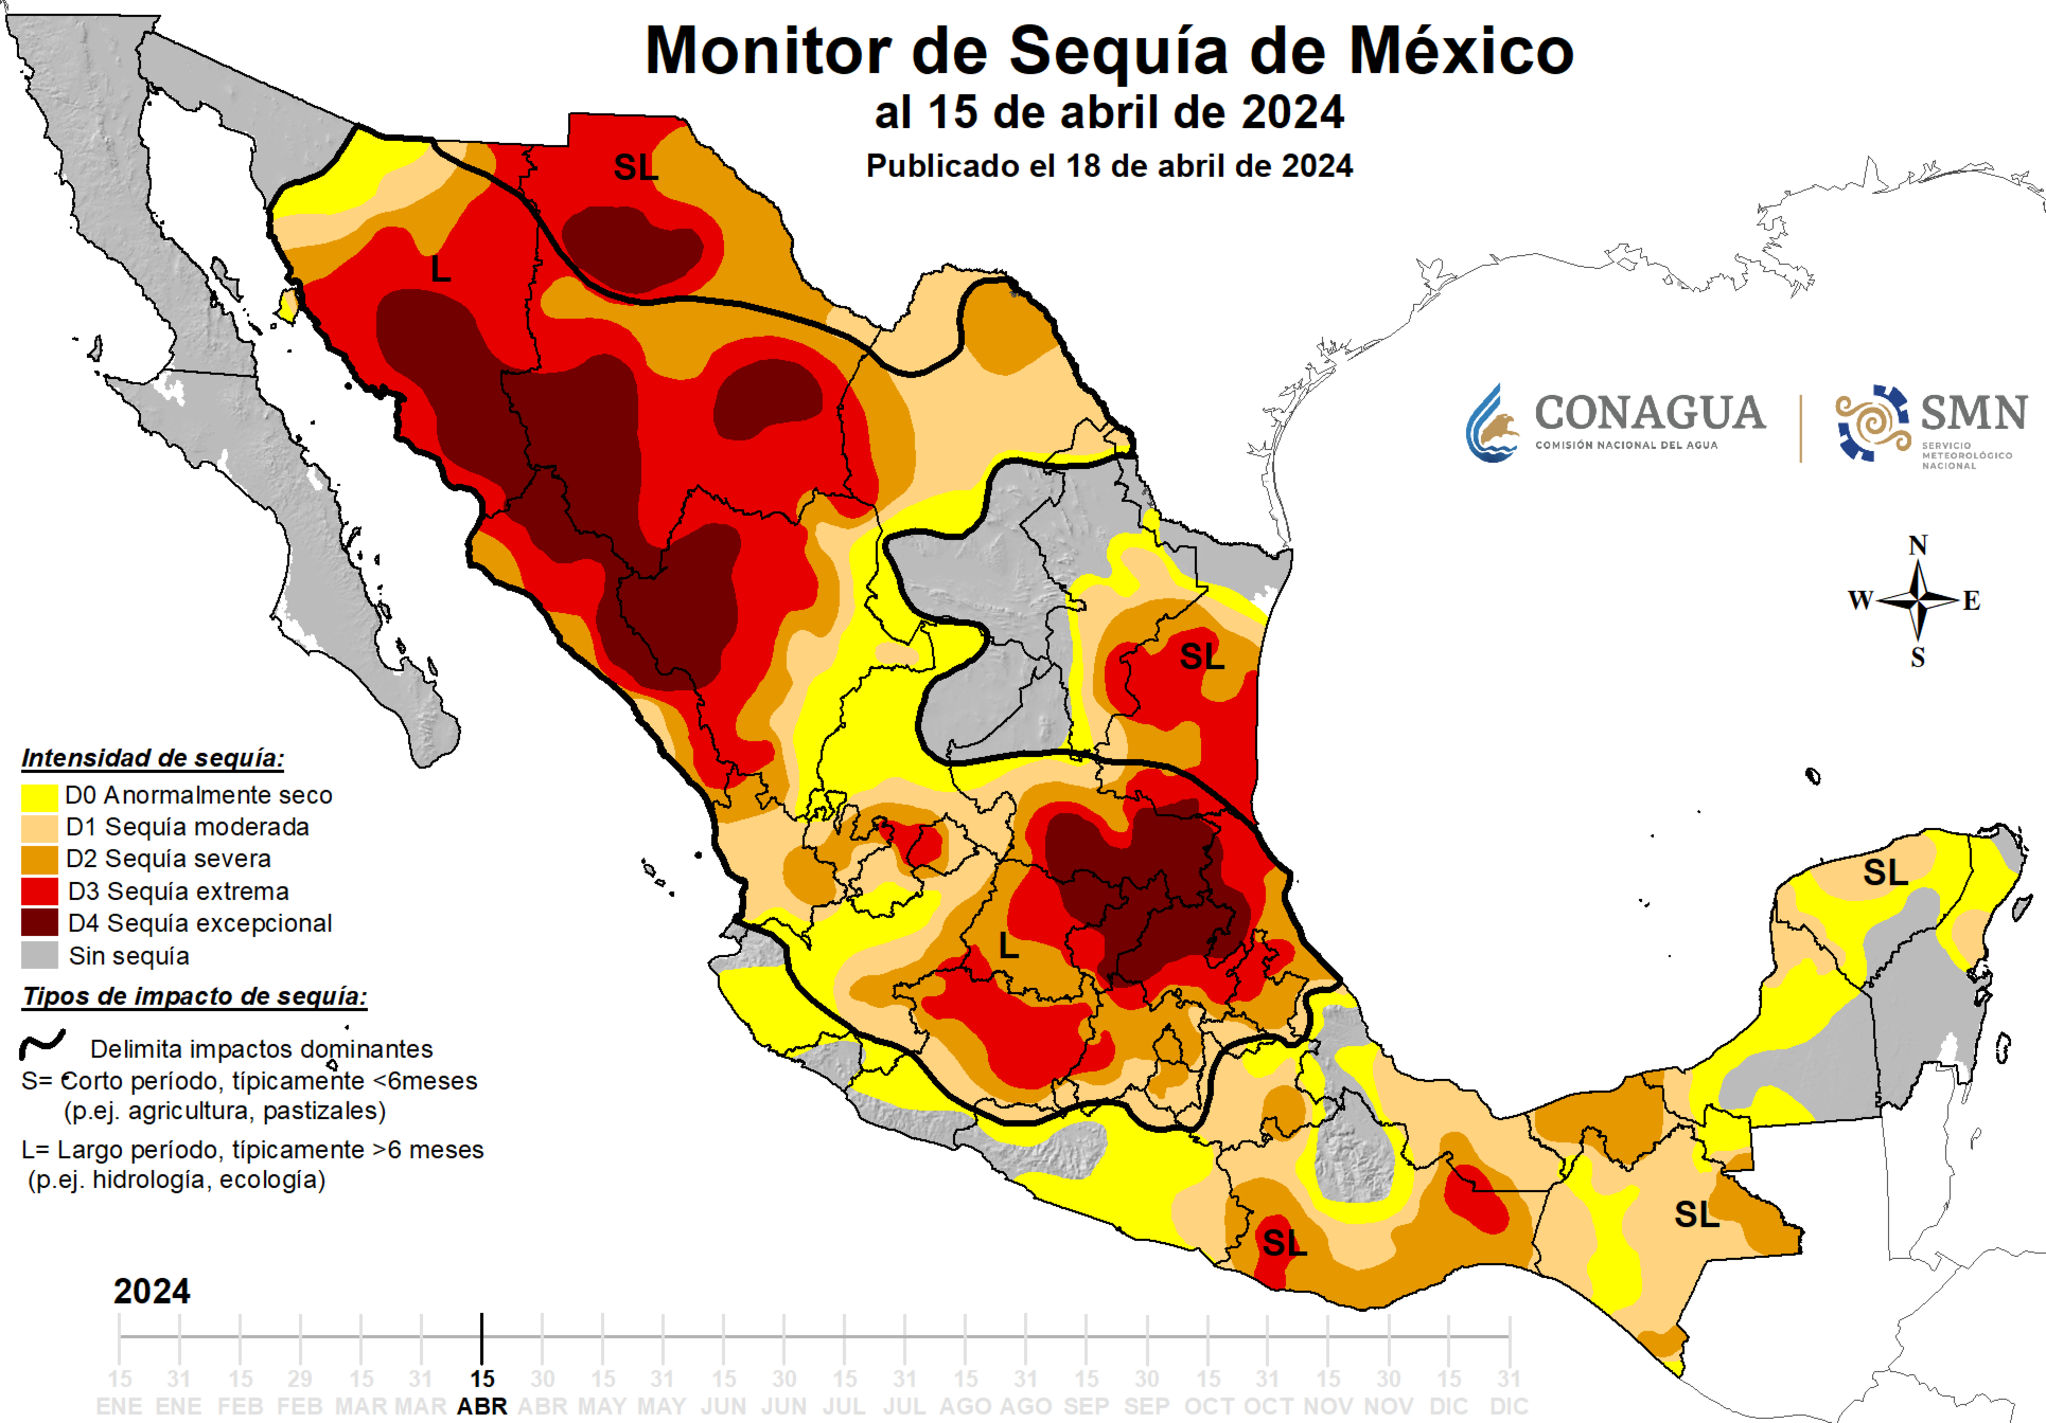
\includegraphics[scale=0.35]{../Images/Sequia.pdf}
	\\\small{Fuente: \cite{CNA2024}}
	\caption{Mapa de México dónde se muestra los niveles de sequía acorde a la intensidad al mes de abril del 2024}\label{fig:sequia}
\end{figure}
La base metodológica del proyecto toma como base los diseños de reactor y experimentos de \cite{Ramalho2003}, donde, los resultados obtenidos fueron utilizados para obtener las constantes cinéticas especificas de los lodos de la \acrshort{PTAR} municipal de Lagos de Moreno para, posteriormente desarrollar un algoritmo de MATLAB, con el cual simular las condiciones de operación del sistema de manera habitual dadas por el usuario y compararlas con las resultantes del sistema real y comparar la efectividad de predicción del algoritmo con respecto al modelo real.
	\section{Justficación}
Los datos presentados en \cite{ODS23} muestran que menos de la mitad del agua residual generada es tratada de manera adecuada, sobre todo en la región hidrológica Lerma-Santiago donde se tiene un deficiente control de las zonas de descarga de las redes colectoras, vertiendo la mayoría en cuerpos de agua superficiales generando problemas sanitarios en poblaciones que no cuentan con plantas potabilizadoras (como es el caso de Lagos de Moreno) \citep{CEAJ2015}.\par
Por tal motivo resulta esencial el fomentar la investigación en técnicas de tratamiento de aguas residuales con vistas a reducir la carga de contaminantes de los cuerpos de agua y generar una recarga artificial de los acuíferos, reduciendo el déficit de agua al que se enfrentan actualmente los acuíferos del país y proponiendo un sistema capaz de satisfacer las necesidades de la población a un bajo coste y con mayor eficiencia de trabajo.\par
Actualmente ya se cuenta con varios modelos, siendo los \gls{ASM} los más representativos y respaldados, contando con varios trabajos de investigación que demuestran la concordancia entre los datos reales y las predicciones generadas por el modelo.\par
\cite{Costa2022}, realiza una comparación entre la aplicación del modelo \acrshort{ASM}1 y la \acrshort{PTAR} de Salamanca España, concluyendo que, aunque el modelo realiza predicciones que llegan a acercarse al resultado in-situ, es necesario que se realicen ajustes a los parámetros \textit{\unichar{"00B5}}$_{H,max}$ y $Y_{H}$ con el fin de conseguir una mejor representación y reducción del error promedio entre los valores de simulación y los datos analizados. También destaca que, si bien el modelado matemático no es capar de predecir la variabilidad generada inevitablemente con respecto a las fluctuaciones en las condiciones de operación a las que son sometidas las comunidades bacterianas dentro del sistema, este proceso sirve para comprender las causas de tales variaciones y como afectan al sistema de manera general con el fin de seguir mejorando el modelo, ya que como lo menciona el autor, el modelo original fue publicado hace mas de 30 años y , aunque se han desarrollado modelos que solventan errores u omisiones del primer modelo, estos están aún lejos de tener errores entre el valor simulado y el analizado in-situ.\par
En otro articulo, \cite{Gernaey04} hablan acerca de las aplicaciones que presenta el modelado en distintos ámbitos, resaltando tres casos:
\begin{enumerate}
	\item \textbf{Simulación con fines educativos:} en dónde se busca que el operador comprenda de forma detallada el funcionamiento del sistema de lodos activados y las implicaciones que generan los cambios en las condiciones operativas, variaciones climáticas y problemas adversos típicos relacionados al ciclo metabólico de las comunidades microbiológicas presentes en el sistema.
	\item \textbf{Simulación con fines de diseño:} buscando en este apartado analizar todos los escenarios posibles para resolver ciertas problemáticas adjuntas a cada caso de estudio, reduciendo costos significativos y tiempo en el escalado entre un sistema de pruebas a nivel laboratorio y la planta piloto. Este punto va de la mano con el siguiente punto, el cual habla de;
	\item \textbf{Simulación para la optimización de procesos:} 
\end{enumerate}
	\section{Objetivos}
\subsection{Objetivo general}
Establecer los parámetros cinéticos de crecimiento, degradación de sustrato, producción de biomasa y consumo de oxígeno óptimos para la remoción de contaminantes que permiten el diseño de sistemas más eficientes y la reducción de los costos de operación, empleando distintas fuentes de alimentación (aguas sintéticas y aguas crudas) a escala de laboratorio utilizando lodos activados.
\subsection{Objetivos particulares}
	\begin{enumerate}
		\item Calcular las constantes de crecimiento microbiano de manera experimental de lodos provenientes de una planta de tratamiento en función
		\item Comparar las diferencias que se generan empleando agua residual de constituyentes conocidos frente a un afluente real.
		\item Simular el proceso de remoción de contaminantes utilizando las herramientas presentes en el programa MATLAB® y las constantes que se generan en el proceso.
	\end{enumerate}

	\section{Materiales}
	\section{Resultados}
	\section{\enspace Discusión}
	\section{Conclusiones}
	\section{Perspectivas}
	\bibliographystyle{apalike}
	\phantomsection
	\addcontentsline{toc}{section}{Referencias}
	\bibliography{../Bibliography/References.bib}
	\clearpage
	\cleardoublepage
	\phantomsection
	\addcontentsline{toc}{section}{Anexos}
	\addtocounter{page}{1}
	\pagenumbering{Roman}
	\pagestyle{Anexos}
	\section*{Anexos}
\subsection*{Prueba de pH Norma Mexicana NMX-AA-008-SCFI-2000}
\begin{center}
	\begin{figure}[h]
		\includegraphics*[scale=0.825]{../Images/nmx-aa-008-scfi-2000_pages-to-jpg-0032.jpg}
	\end{figure}
\end{center}
\clearpage
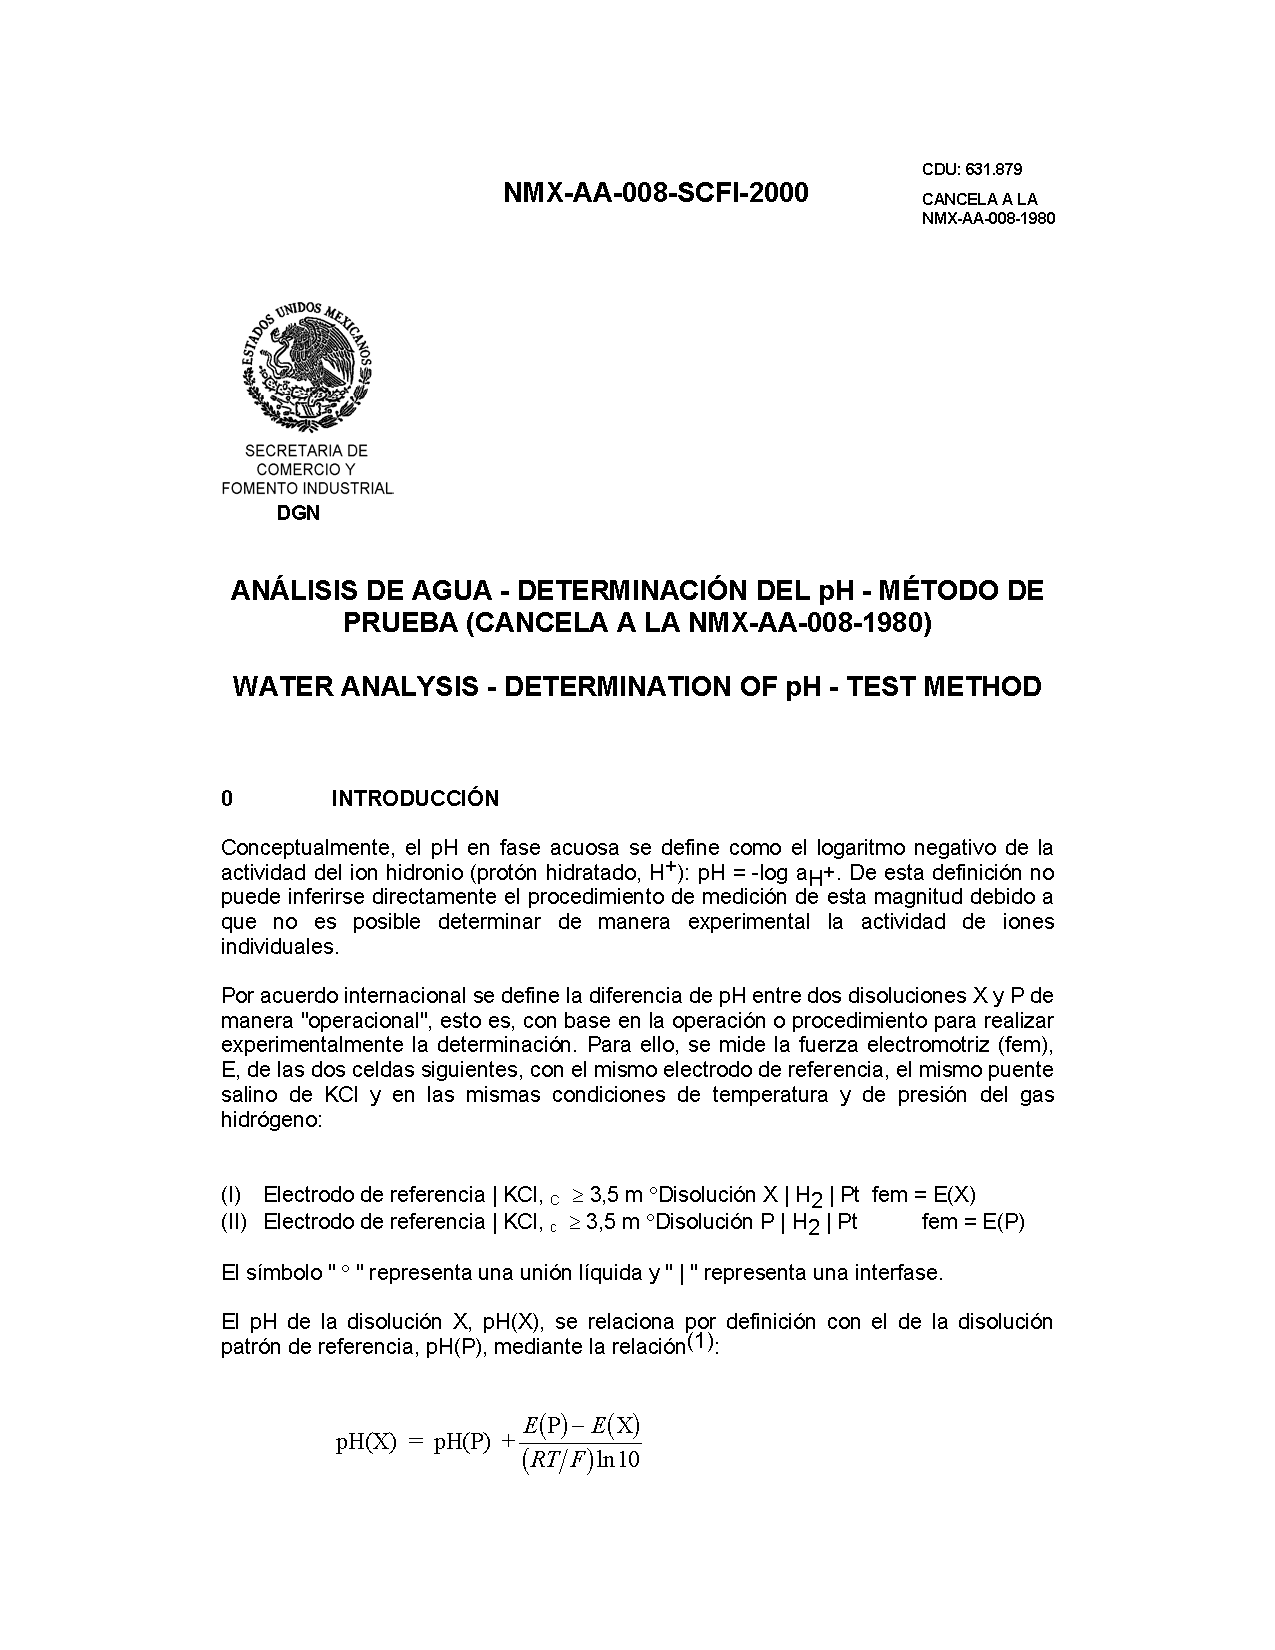
\includepdf[pages=-30, pagecommand={}]{../Documents/nmx-aa-008-scfi-2000}
	\clearpage
	\cleardoublepage
	\phantomsection
	\pagestyle{Sigla}
	\addcontentsline{toc}{section}{Siglas}
	\printglossary[type=\acronymtype]
	\clearpage
	\phantomsection
	\pagestyle{Glosario}
	\addcontentsline{toc}{section}{Glosario}
	\setglossarystyle{altlistgroup}
	\printglossary
\end{document}